%\documentclass[letterpaper, 10pt]{sigcomm-alternate}

\documentclass[peerreview, a4paper, 7pt]{IEEEtran}
%\documentclass[a4paper, 10pt]{IEEEtran}
%\documentclass{scrreprt}
\usepackage{times}
\usepackage{alltt}
\usepackage{graphicx}
\usepackage{alltt}
\usepackage{colortbl}
\usepackage[dvipsnames]{xcolor}

%\usepackage{color}
% \usepackage{caption2}
%\usepackage{subfigure}
%\usepackage{graphicx}
%\usepackage{colortbl}
%\usepackage[dvipsnames]{xcolor}
% \usepackage{ulem}

\usepackage{hyperref}

\pagenumbering{arabic}


%\ifx\pdfoutput\undefined
%\usepackage[pdfpagemode=none, pdfstartview=FitH, colorlinks=true, urlcolor=black, linkcolor=black, citecolor=black]{hyperref}
%\else
%\usepackage[pdftex, pdfpagemode=none, pdfstartview=FitH, colorlinks=true, urlcolor=black, linkcolor=black, citecolor=black, pdftex]{hyperref}
%\fi

\ifx\HCode\UnDef\else\hypersetup{tex4ht}\fi

%% Editorial work
% \newcommand{\purge}[1]{\textcolor{red}{\sout{#1}}}
% \newcommand{\add}[1]{\textcolor{blue}{#1}}

%%% End of editorial work.


 
\renewcommand{\em}[1]{\textit{#1}}
\begin{document}

\title{Software and Firmware Updates with the OMA LWM2M Protocol}

\author{\authorblockN{Hannes Tschofenig\authorrefmark{1}\\}
\authorblockA{\authorrefmark{3}ARM Limited, 
Email: hannes.tschofenig@arm.com\\}
\thanks{\textsc{Position paper for the 'Internet of Things Software Update Workshop (IoTSU)'~\cite{IOTSU}, 13$^{th}$ and 14$^{th}$ June 2016, Dublin, Ireland.} The content of this document describes the views of the author.}
}

\date{\today}

\maketitle


\section{Abstract}


The Lightweight Machine-to-Machine (LWM2M)~\cite{lwm2m} protocol has been developed by the Open Mobile Alliance (OMA) to provide a number of device management functions, including software and firmware updates. With mbed Client and mbed Connector, ARM has implemented LWM2M and offers it to developers. This position paper describes what functionality has been standardized in LWM2M for software and firmware updates and what open issues exist. 

\section{LWM2M Overview}
\label{lwm2m}

The high-level architecture of LWM2M is shown in Figure~\ref{lwm2m-architecture-figure} where the LWM2M client, running on an IoT device, interacts with an LWM2M server. LWM2M v1.0 supports  CoAP over both UDP and SMS. The protocol assumes the use of DTLS for communication security and offers various RESTful APIs (interfaces) that allow communicating structured data. The data is organized in the form of objects that contain resources. The detailed structure of the data model has been the subject of a separate position paper published in the IoT Semantic Interoperability Workshop 2016; see~\{cite{ipso-iotsi-paper}. 

\begin{figure}[!htbp]
 \centering
 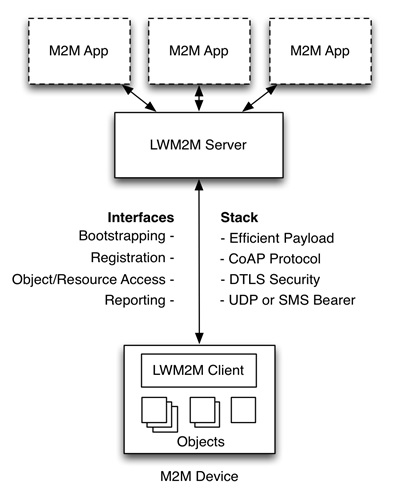
\includegraphics[scale=0.50]{lwm2m-architecture.jpg}
 \caption{LWM2M Architecture.}
 \label{lwm2m-architecture-figure}
\end{figure}

A number of objects have been standardized already to allow the exchange of data between an IoT device and the server-side infrastructure. This communication is bi-directional and allows the server to obtain sensor readings, control actuators and so on. The same object model is used for the interactions. A full list of the already standardized objects can be found at a registry maintained by the OMA~\cite{OMNA}. This registry contains a firmware object as well as a software management object. The functionality of the two is described in the subsections below.

\subsection{Firmware Object} 
The object definition of the firmware object can be found at~\cite{firmware-object}. It includes a number of resources, namely 
\begin{enumerate}
\item The firmware package itself or a URI pointing to it. The idea of using a URI is to allow a server to instruct a client to download the firmware from another source. 
\item Various resources to expose the protocol interaction and the result of the firmware update operation. For example, the Update Result resource allows an LWM2M client to expose information about the reason for a failed software update, or that the update has been performed successfully. 
\end{enumerate}

The process for providing a firmware to a device is supposed to happen in two stages: the download of the firmware image, and then the execution of the update. An update can only be executed when the device has successfully downloaded the firmware image (and presumably took the necessary verification steps) and has transitioned into the 'Downloaded' state. 

The object definition indicates that only a single firmware object can be present on a device. Furthermore, there is no meta-data in the object definition about the content of the firmware package. 

\subsection{Software Management Object}
Since the firmware object was seen as too basic, an extended version - called software management object - was developed. The object definition of the software management object is not included in the main LWM2M specification, but has instead been published as a separate specification~\cite{SwMgmt}. It defines two objects: the Software Component object (with object ID 14) and the Software Management object (with object ID 9). 

The added functionality provided by these two objects aims to focus on devices where multiple software packages are installed. Similarly to the firmware update procedure, the server can push a software package or a URI to a software package. If the client needs authentication to download the software package over a URI, the server may also provision a username/password to the client. Unlike the firmware update procedure, in software management it is also necessary to activate software after it has been installed. Software management also supports deactivating and removing a software package. 

The Software Management object also defines basic meta-data about the name and the version of the package and contains one or more links to Software Component objects. Figure~\ref{software-management-figure} illustrates the relationship between the two objects. 

\begin{figure}[!htbp]
 \centering
 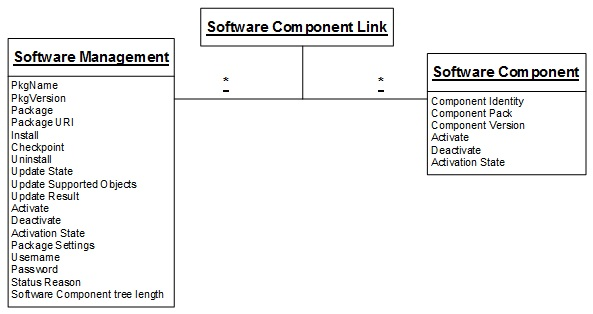
\includegraphics[scale=0.50]{software-management.jpg}
 \caption{Software Management.}
 \label{software-management-figure}
\end{figure}

As shown, the software management object may contain of one or more software components. In addition to the multiple software components a device may also have multiple software management objects. 

\section{What are we trying to standardize?}
\label{what}

The OMA work on software and firmware updates, as two independent solutions, hints to the fuzzy definition of the Internet of Things. IoT devices, in ARM jargon, may be devices that run Cortex A class processors and are therefore able to run general purpose operating systems, such as Arch Linux, since they are equipped with a memory management unit, use more powerful processors, and also have more RAM and flash memory. Devices with such operating systems have, for a long time, been using sophisticated software update mechanisms (such as Pacman). Software has also been provided by different developers, and thanks to the isolation techniques offered by the hardware and modern operating systems, a failure in one software typically does not impact other software components (from a security point of view). Often software update mechanisms on these devices allow updates to be obtained from various sources. 

\textsc{Question}: Do we need additional software update standards for these A-class devices?

To make the question more complicated, many A-class type processors offer a hardware security features called Trusted Execution Environments (TEEs)~\cite{TEE}. These TEEs provide a separation between the full blown, general purpose operating system and a real-time operating system. The two sides are often referred to as "normal world" and "secure world". The purpose of the separation is to place security-sensitive components in the smaller, better audited, and more tightly controlled real-time operating system - and to use hardware features to control the transition between the two worlds. Software/firmware updates for the secure world are often very different, technically and operationally, from the update mechanism used in the normal world.

\textsc{Question}: Is there a need for a software/firmware update mechanism for the secure world on A-class-like devices? 

In the move from the Cortex A-class devices to the more constrained Cortex M-class devices, a different software development practice has been established. While software has gotten more and more complex (with the desire to connect to various Internet services), only a single firmware image is uploaded to the M-class IoT device. This image typically contains software libraries from various sources, and may even contain binary images that have been provided by silicon manufacturers. This means that in some cases the developer may not have access to the full source code, but instead has to link a binary to his or her code\footnote{An example of this approach can be seen with the Bluetooth Low Energy (BLE) microcontrollers offered by Nordic Semiconductor, such as the Nordic nRF51-DK~\cite{nRF51-DK}. Nordic thereby offers the BLE protocol stacks as so-called SoftDevices for download. SoftDevices are pre-compiled, pre-linked binary files, which subsequently need to be linked to the actual application code (such as a BLE peripheral providing the features of a heart-rate monitor.)}.

While some companies have been experimenting with Java Virtual Machines - or similar sandboxing techniques - to allow downloading software components from different sources, these efforts typically challenge the very nature of the M-class devices. These devices are supposed to be cheap, purpose-built, energy efficient and equipped with limited resources (RAM, flash, etc).  

\textsc{Question}: What are the minimum requirements for firmware updates for such M-class devices? What components need to be standardized to make it easier for developers to improve their IoT software's security?

Security has been an important consideration for all Internet connected devices and TEEs were introduced to A-class devices (with ARM TrustZone) many years ago. In November 2015, ARM made a technology launch of TrustZone for v8-M~\cite{Trustzone} and thereby completed the v8 architecture for application (A), real-time (R), and microcontroller (M) devices. It remains to be seen whether the developer experience for devices using TrustZone for v8-M and v8-A will be similar or very different. Other hardware security features may impose a certain deployment or developer model.

\textsc{Question}: How do hardware security features for embedded devices impact firmware update mechanisms?

\section{Open Issues with LWM2M}
\label{open-issues}
The introduction to LWM2M mentioned functionality that has not been standardized, and there may be good reasons for leaving certain functionality either out of scope or subject to proprietary implementations. The following subsections highlight a few of the identified open issues. 

\subsection{Choice of Transport and Fragmentation}

Firmware updates may potentially be large (over 100 KiB for a Cortex M-based device). Although the transport of software and firmware updates has been standardized with LWM2M, the use of CoAP - which runs on top of UDP - quickly leads to problems. First, UDP has a maximum size limit of about 64 KiB. Second, transmitting UDP messages that are larger than the path MTU size leads to fragmentation of these messages at the lower layers, typically IP. It may also lead to fragmentation at the adaptation layer. 

It turns out that CoAP over TCP, as well as the blockwise transfer developed for CoAP more recently in the IETF CoRE working group, can help mitigate these problems. Unfortunately, the LWM2M v1.0 does not support these newer CoAP extensions. As a consequence, software/firmware updates with file sizes larger than ~64 KiB are not supported. Furthermore, the performance of any software/firmware update using CoAP alone (without utilizing these extensions) over low power radio technologies (such as IEEE 802.16.4, or the recently developed low power wide area networks) will be significantly degraded due to the interplay between packet loss and the fragmentation behavior at the IP or adaptation layer.

When firmware images are distributed to a large number of devices, the caching capabilities of CoAP and other protocols, including multicast support, may turn out to be useful - but they are not discussed in the LWM2M specification.

Ideally, a firmware distribution mechanism should offer flexible transport to allow it to be used over a number of different technologies. Some of these radio technologies are lossy, requiring re-transmission of a subset of the transmitted data. Efficiency of the firmware distribution is important, because a firmware update of a device running on a coin-cell battery can easily drain half of the battery capacity. 

\subsection{Meta-Data}

The LWM2M firmware object contains no meta-data about the firmware image itself, and the Software Management object only contains a minimal amount of meta-data. Quite naturally, the question arises what type of meta-data needs to be standardized as part of the data model. For example, the firmware object is only available as a single instance, and this raises the question about the possible implications for devices that have multiple microcontrollers, each of which will need an independent update. While this questions appears to be a hardware/software implementation design detail it does, in fact, have an impact on the data model. Would it be useful to capture the details of the internals of an IoT device to be able to communicate which microcontroller needs to be updated, or is this a detail only the hardware developer needs to care about? 

Firmware images come in different formats - as Portable Executable (PE) and Executable and Linking Format (ELF) - they may be compressed or come in form of diffs, they may consist of a single file or combined into multiple files. While it is certainly helpful to indicate the content type of the payloads being communicated, is it useful for developers to settle on one or a few popular formats and compression techniques?

\subsection{Application Layer Security}

LWM2M offers protecting the transmission of software and firmware updates via DTLS, and communication layer security is definitely a viable option for protecting these sensitive payloads in flight, as well as to authenticate and authorize the endpoints. When firmware images are cached in other locations (for example, distributed to other servers, cached by proxies, or used in a store-and-forward fashion), it may be necessary to offer application layer security protection (e.g., message authentication codes, digital signatures, and - potentially - confidentiality protection) either as a replacement for communication security or in addition. Regarding serialization formats, a number of choices do exist already, such as ASN.1/CMS, JSON/JOSE, and CBOR/COSE. While they are all fairly similar in functionality, there are still subtle differences due to their histories. What technique is most favored by industry players? 

Since all these mechanisms are very flexible, different types of credentials are supported (e.g., symmetric keys, raw public keys and X.509 certs), with a variety of different cryptographic algorithms. Is there some scope to increase interoperability and at the same time keep the code size as well as memory footprint at an acceptable level? To verify these protected payloads (and also for the use of communication security) the device needs to be provisioned with trust anchors, or other keying material that allow verification. These types of credentials may be used to force a certain deployment choice.

\section{Summary}
This document starts with an overview of the functionality provided by LWM2M in Section~\ref{lwm2m}. Section~\ref{what} then raises the question about where additional standardization work is needed. The answer will depend on the type of IoT device being dealt with and the level of interoperability the community desires. Finally, a couple of open issues are identified in the context of the LWM2M firmware/software update mechanism. 

By reaching out to the wider Internet community we hope to get more input on the currently deployed software/firmware update procedures. The most important building blocks and the best current practices should be standardized. These could serve as a valuable toolbox for developers trying to bring IoT devices to the market faster.

Besides the more technical aspects raised in the write-up above, there have been various concerns expressed by the Federal Trade Commission (FTC)~\cite{FTC} as well as by the Article 29 Working Party of the European Commission~\cite{Article29WP}. The concerns range from how end users should grant permissions for software updates (while on the other hand updating software as quickly as possible) to questions like 'Should modern refrigerators have a shelf-life, much like the food contained within?'~\cite{ShelfLife}. While these questions are important and need to be answered by the wider community, the author believes that the IOTSU workshop~\cite{IOTSU} is less likely to make progress on answering these questions.  

\bibliographystyle{IEEEtran}
% \bibliographystyle{acmtrans}
\bibliography{paper}


\end{document}

